%beamer

% Comment/uncomment this line to toggle handout mode
\newcommand{\handout}{}

%% Beamer-Klasse im korrekten Modus
\ifdefined \handout
\documentclass[handout]{beamer} % Handout mode
\else
\documentclass{beamer}
\fi

%% UTF-8-Encoding
\usepackage[utf8]{inputenc}

\input{../framework/gbi-macros}
\usepackage[blue]{../framework/thwregex}
\usepackage{environ}
\usepackage{bm}
\usepackage{calc}
\usepackage{varwidth}
\usepackage{wasysym}
\usepackage{mathtools}


% Das ist der KIT-Stil
%\usepackage{../TutTexbib/beamerthemekit}
\usepackage[deutsch,titlepage0]{../framework/KIT/beamerthemeKITmod}
\TitleImage[width=\titleimagewd]{../figures/titlepage.jpg}
%\usetheme[deutsch,titlepage0]{KIT}

% Include PDFs
\usepackage{pdfpages}

% Libertine font (Original GBI font)
\usepackage{libertine}
%\renewcommand*\familydefault{\sfdefault}  %% Only if the base font of the document is to be sans serif

% Nicer math symbols
\usepackage{eulervm}
%\usepackage{mathpazo}
\renewcommand\ttdefault{cmtt} % Computer Modern typewriter font, see lecture slides.

\usepackage{csquotes}

%%%%%%

%% Schönere Schriften
\usepackage[TS1,T1]{fontenc}

%% Bibliothek für Graphiken
\usepackage{graphicx}

%% der wird sowieso in jeder Datei gesetzt
\graphicspath{{../figures/}}

%% Anzeigetiefe für Inhaltsverzeichnis: 1 Stufe
\setcounter{tocdepth}{1}

%% Hyperlinks
\usepackage{hyperref}
% I don't know why, but this works and only includes sections and NOT subsections in the pdf-bookmarks.
\hypersetup{bookmarksdepth=subsection} 

%\usepackage{lmodern}
\usepackage{colortbl}
\usepackage[absolute,overlay]{textpos}
\usepackage{listings}
\usepackage{forloop}
%\usepackage{algorithmic} % PseudoCode package 

\usepackage{tikz}
\usetikzlibrary{matrix}
\usetikzlibrary{arrows.meta}
\usetikzlibrary{automata}
\usetikzlibrary{tikzmark}
\usetikzlibrary{positioning}

% Why has no-one come up with this yet? I mean, seriously. -.-
\tikzstyle{loop below right} = [loop, out=-60,in=-30, looseness=7]
\tikzstyle{loop below left} = [loop, out=-150,in=-120, looseness=7]
\tikzstyle{loop above right} = [loop, out=60,in=30, looseness=7]
\tikzstyle{loop above left} = [loop, out=150,in=120, looseness=7]
\tikzstyle{loop right below} = [loop below right]
\tikzstyle{loop left below} = [loop below left]
\tikzstyle{loop right above} = [loop above right]
\tikzstyle{loop left above} = [loop above left]

% Needed for gbi-macros
\usepackage{xspace}

%%%%%%

%% Verbatim
\usepackage{moreverb}

%%%%%%%%%%%%%%%%%%%%%%%%%%%%%%%%%%%% Copy end

%% Tabellen
\usepackage{array}
\usepackage{multicol}
\usepackage{hhline}

%% Bibliotheken für viele mathematische Symbole
\usepackage{amsmath, amsfonts, amssymb}

%% Deutsche Silbentrennung und Beschriftungen
\usepackage[ngerman]{babel}

\usepackage{kbordermatrix}

% kbordermatrix settings
\renewcommand{\kbldelim}{(} % Left delimiter
\renewcommand{\kbrdelim}{)} % Right delimiter

\input{../config.tex}



% define custom \handout command flag if handout mode is toggled  #DirtyAsHellButWell...
\only<beamer:0>{\def\handout{}} %beamer:0 == handout mode

\newcommand{\R}{\mathbb{R}}
\newcommand{\N}{\mathbb{N}}
\newcommand{\Z}{\mathbb{Z}}
\newcommand{\Q}{\mathbb{Q}}
\newcommand{\BB}{\mathbb{B}}
\newcommand{\C}{\mathbb{C}}
\newcommand{\K}{\mathbb{K}}
\newcommand{\G}{\mathbb{G}}
\newcommand{\nullel}{\mathcal{O}}
\newcommand{\einsel}{\mathds{1}}
\newcommand{\Pot}{\mathcal{P}}
\renewcommand{\O}{\text{O}}

\def\word#1{\hbox{\textcolor{blue}{\texttt{#1}}}}
\let\literal\word
\def\mword#1{\hbox{\textcolor{blue}{$\mathtt{#1}$}}}  % math word
\def\sp{\scalebox{1}[.5]{\textvisiblespace}}
\def\wordsp{\word{\sp}}

%\newcommand{\literal}[1]{\textcolor{blue}{\texttt{#1}}}
\newcommand{\realTilde}{\textasciitilde \ }
\newcommand{\setsize}[1]{\ensuremath{\left\lvert #1 \right\rvert}}
\newcommand{\size}[1]{\setsize{#1}}  % Shame on you, TeXStudio...
\newcommand{\set}[1]{\left\{#1\right\}}
\newcommand{\tuple}[1]{\left(#1\right)}
\newcommand{\normalvar}[1]{\text{$#1$}}

% Modified by DJ
\let\oldemptyset\emptyset
\let\emptyset\varnothing % proper emptyset

\newcommand{\boder}{\ensuremath{\mathbin{\textcolor{blue}{\vee}}}\xspace}
\newcommand{\bund}{\ensuremath{\mathbin{\textcolor{blue}{\wedge}}}\xspace}
\newcommand{\bimp}{\ensuremath{\mathrel{\textcolor{blue}{\to}}}\xspace}
\newcommand{\bgdw}{\ensuremath{\mathrel{\textcolor{blue}{\leftrightarrow}}}\xspace}
\newcommand{\bnot}{\ensuremath{\textcolor{blue}{\neg}}\xspace}
\newcommand{\bone}{\ensuremath{\textcolor{blue}{1}}\text{}}
\newcommand{\bzero}{\ensuremath{\textcolor{blue}{0}}\text{}}
\newcommand{\bleftBr}{\ensuremath{\textcolor{blue}{\texttt{(}}}\text{}}
\newcommand{\brightBr}{\ensuremath{\textcolor{blue}{\texttt{)}}}\text{}}

% Fix of \b... commands:

\renewcommand{\boder}{\alor}
\renewcommand{\bund}{\aland}
\renewcommand{\bimp}{\alimpl}
\renewcommand{\bgdw}{\aleqv}
\renewcommand{\bnot}{\alnot}
\renewcommand{\bleftBr}{\alka}
\renewcommand{\brightBr}{\alkz}
\newcommand{\alA}{\word A}
\newcommand{\alB}{\word B}
\newcommand{\alC}{\word C}

\newcommand{\plB}{\plfoo{B}}
\newcommand{\plE}{\plfoo{E}}

\newcommand{\summe}[2]{\sum\limits_{#1}^{#2}}
\newcommand{\limes}[1]{\lim\limits_{#1}}

%\newcommand{\numpp}{\advance \value{weeknum} by -2 \theweeknum \advance \value{weeknum} by 2}
%\newcommand{\nump}{\advance \value{weeknum} by -1 \theweeknum \advance \value{weeknum} by 1}

\newcommand{\mycomment}[1]{}
\newcommand{\Comment}[1]{}

%% DISCLAIMER START 
% It is INSANELY IMPORTANT NOT TO DO THIS OUTSIDE BEAMER CLASS! IN ARTCILE DOCUMENTS, THIS IS VERY LIKELY TO BUG AROUND!
\makeatletter%
\@ifclassloaded{beamer}%
{
	% TODO 
	% no time... later.   (= never -.-)
	% redefine section to ignore multiple \section calls with the same title
}%
{
	\errmessage{ERROR: section command redefinition outside of beamer class document! Please contact the author of this code or read the F-ing disclaimer.}
}%
\makeatother%
%% DISCLAIMER END

\newcounter{abc}
\newenvironment{alist}{
  \begin{list}{(\alph{abc})}{
      \usecounter{abc}\setlength{\leftmargin}{8mm}\setlength{\labelsep}{2mm}
    }
}{\end{list}}


\newcommand{\stdarraystretch}{1.20}
\renewcommand{\arraystretch}{\stdarraystretch}  % for proper row spacing in tables

\newcommand{\morescalingdelimiters}{   % for proper \left( \right) typography
	\delimitershortfall=-1pt  
	\delimiterfactor=1
}

\newcommand{\centered}[1]{\vspace{-\baselineskip}\begin{center}#1\end{center}\vspace{-\baselineskip}}

% for \implitem and \item[bla] stuff to look right:
\setbeamercolor*{itemize item}{fg=black}
\setbeamercolor*{itemize subitem}{fg=black}
\setbeamercolor*{itemize subsubitem}{fg=black}

\setbeamercolor*{description item}{fg=black}
\setbeamercolor*{description subitem}{fg=black}
\setbeamercolor*{description subsubitem}{fg=black}

\renewcommand{\qedsymbol}{\textcolor{black}{\openbox}}

\renewcommand{\mod}{\mathop{\textbf{mod}}}
\renewcommand{\div}{\mathop{\textbf{div}}}

\newcommand{\ceil}[1]{\left\lceil#1\right\rceil}
\newcommand{\floor}[1]{\left\lfloor#1\right\rfloor}
\newcommand{\abs}[1]{\left\lvert #1 \right\rvert}
\newcommand{\Matrix}[1]{\begin{pmatrix} #1 \end{pmatrix}}
\newcommand{\braced}[1]{\left\lbrace #1 \right\rbrace}

% "something" placeholder. Useful for repairing spacing of operator sections, like `\sth = 42`.
\def\sth{\vphantom{.}}

\def\fract#1/#2 {\frac{#1}{#2}} % ! Trailing space is crucial!
\def\dfract#1/#2 {\dfrac{#1}{#2}} % ! Trailing space is crucial!

\newcommand{\Mid}{\;\middle|\;}

\let\after\circ



\def\·{\cdot}
\def\*{\cdot}
\def\?>{\ensuremath{\rightsquigarrow}}  % Fuck you, Latex
\def\~~>{\ensuremath{\rightsquigarrow}}  

\newcommand{\tight}[1]{{\renewcommand{\arraystretch}{0.76} #1}}
\newcommand{\stackedtight}[1]{\renewcommand{\arraystretch}{0.76} \begin{matrix} #1 \end{matrix} }
\newcommand{\stacked}[1]{\begin{matrix} #1 \end{matrix} }
\newcommand{\casesl}[1]{\delimitershortfall=0pt  \left\lbrace\hspace{-.3\baselineskip}\begin{array}{ll} #1 \end{array}\right.}
\newcommand{\casesr}[1]{\delimitershortfall=0pt  \left.\begin{array}{ll} #1 \end{array}\hspace{-.3\baselineskip}\right\rbrace}
\newcommand{\caseslr}[1]{\delimitershortfall=0pt  \left\lbrace\hspace{-.3\baselineskip}\begin{array}{ll} #1 \end{array}\hspace{-.3\baselineskip}\right\rbrace}

\def\q#1uad{\ifnum#1=0\relax\else\quad\q{\the\numexpr#1-1\relax}uad\fi}
% e.g. \q1uad = \quad, \q2uad = \qquad etc.

\newcommand{\qqquad}{\q3uad}
\newcommand{\minusquad}{\hspace{-1em}}

%% Placeholder utils
% \§{#1}   Saves #1 as placeholder and prints it
% \.       Prints an \hphantom with the size of the recalled placeholder.
\def\indentstring{}
\def\§#1{\def\indentstring{#1}#1}
\def\.{{$\hphantom{\text{\indentstring}}$}}
%% Placeholder utils end

\newcommand{\impl}{\ifmmode\ensuremath{\mskip\thinmuskip\Rightarrow\mskip\thinmuskip}\else$\Rightarrow$\fi\xspace}
\newcommand{\Impl}{\ifmmode\implies\else$\Longrightarrow$\fi\xspace}

\newcommand{\derives}{\Rightarrow}

\newcommand{\gdw}{\ifmmode\mskip\thickmuskip\Leftrightarrow\mskip\thickmuskip\else$\Leftrightarrow$\fi\xspace}
\newcommand{\Gdw}{\ifmmode\iff\else$\Longleftrightarrow$\fi\xspace}

% Legacy code from the algo tutorial slides. Perhaps useful. Try with care.
\mycomment{
	\newcommand{\impl}{\ifmmode\ensuremath{\mskip\thinmuskip\Rightarrow\mskip\thinmuskip}\else$\Rightarrow$\xspace\fi}  
	\newcommand{\Impl}{\ifmmode\implies\else$\Longrightarrow$\xspace\fi}
	
	\newcommand{\gdw}{\ifmmode\mskip\thickmuskip\Leftrightarrow\mskip\thickmuskip\else$\Leftrightarrow$\xspace\fi}
	\newcommand{\Gdw}{\ifmmode\iff\else$\Longleftrightarrow$\xspace\fi}
}
	
\newcommand{\gdwdef}{\ifmmode\mskip\thickmuskip:\Leftrightarrow\mskip\thickmuskip\else:$\Leftrightarrow$\xspace\fi}
\newcommand{\Gdwdef}{\ifmmode\mskip\thickmuskip:\Longleftrightarrow\mskip\thickmuskip\else:$\Longleftrightarrow$\xspace\fi}

\newcommand{\symbitemnegoffset}{\hspace{-.5\baselineskip}}
\newcommand{\implitem}{\item[\impl\symbitemnegoffset]}
\newcommand{\Implitem}{\item[\Impl\symbitemnegoffset]}


\newcommand{\forcenewline}{\mbox{}\\}

\newcommand{\bfalert}[1]{\textbf{\alert{#1}}}
\let\elem\in   % I'm a Haskell freak. Don't judge me. :P


\def\|#1|{\text{\normalfont #1}}  % | steht für senkrecht (anstatt kursiv wie sonst im math mode)


% proper math typography
\newcommand{\functionto}{\longrightarrow}
\renewcommand{\geq}{\geqslant}
\renewcommand{\leq}{\leqslant}
\let\oldsubset\subset
\renewcommand{\subset}{\subseteq} % for all idiots out there using subset

\newenvironment{threealign}{%
	\[
	\begin{array}{r@{\ }c@{\ }l}
}{%
	\end{array}	
	\]
}

\newcommand{\concludes}{ \\ \hline  }
\newcommand{\deduction}[1]{
	\begin{varwidth}{.8\linewidth}
		\begin{tabular}{>{$}c<{$}}
			#1
		\end{tabular}
	\end{varwidth}	
}

\definecolor{hoareorange}{rgb}{1,.85,.6}
\newcommand{\hoareassert}[1]{\setlength{\fboxsep}{1pt}\setlength{\fboxrule}{-1.4pt}\fcolorbox{white}{hoareorange}{\ensuremath{\{\;#1\;\}}}\setlength\fboxrule{\defaultfboxrule}\setlength{\fboxsep}{3pt}}

\newcommand{\mailto}[1]{\href{mailto:#1}{{\textcolor{blue}{\underline{#1}}}}}
\newcommand{\urlnamed}[2]{\href{#2}{\textcolor{blue}{\underline{#1}}}}
\renewcommand{\url}[1]{\urlnamed{#1}{#1}}

\newcommand{\hanging}{\hangindent=0.7cm}
\newcommand{\indented}{\hanging}


% \hstretchto prints #2 left-aligned into a box of the width of #1
\def\hstretchto#1#2{%
	\mbox{}\vphantom{#2}\rlap{#2}\hphantom{#1}%
}

\def\vstretchto#1#2{%
	\mbox{}\hphantom{#2}\smash{#2}\vphantom{#1}%
}

% \hstretchtocentered prints #2 centered into a box of the width of #1
\def\hstretchtocentered#1#2{%
	\mbox{}\vphantom{#2}\scalebox{0.5}{\hphantom{#1}}\clap{#2}\scalebox{0.5}{\hphantom{#1}}%
}

% vertical centering
\newcommand{\vertcenter}[1]{%
	\ensuremath{\vcenter{\hbox{#1}}}%
}


%requires \thisyear to be defined (s. config.tex)!
\edef\nextyear{\the\numexpr\thisyear+1\relax}


% --- \frameheight constant ---
\newlength\fullframeheight
\newlength\framewithtitleheight
\setlength\fullframeheight{.92\textheight}
\setlength\framewithtitleheight{.86\textheight}

\newlength\frameheight
\setlength\frameheight{\fullframeheight}

\let\frametitleentry\relax
\let\oldframetitle\frametitle
\def\newframetitle#1{\global\def\frametitleentry{#1}\if\relax\frametitleentry\relax\else\setlength\frameheight{\framewithtitleheight}\fi\oldframetitle{#1}}
\let\frametitle\newframetitle

\def\newframetitleoff{\let\frametitle\oldframetitle}
\def\newframetitleon{\let\frametitle\newframetitle}
% --- \frameheight constant end ---

\newcommand{\fakeframetitle}[1]{%
	\vspace{-2.05\baselineskip}%
	{\Large \textbf{#1}} \\%
	\smallskip
}



\newenvironment{headframe}{\Huge THIS IS AN ERROR. PLEASE CONTACT THE ADMIN OF THIS TEX CODE. (headframe env def failed)}{}
\RenewEnviron{headframe}[1][]{
	\begin{frame}\frametitle{\ }
		\centering
		\Huge\textbf{\textsc{\BODY} \\
		}
		\Large {#1}
		\frametitle{\ }
	\end{frame}
}


\makeatletter
% Provides color if undefined.
\newcommand{\colorprovide}[2]{%
	\@ifundefinedcolor{#1}{\colorlet{#1}{#2}}{}}
\makeatother


\colorprovide{lightred}{red!30}
\colorprovide{lightgreen}{green!40}
\colorprovide{lightyellow}{yellow!50}
\colorprovide{lightblue}{blue!10}
\colorprovide{beamerlightred}{lightred}
\colorprovide{beamerlightgreen}{lightgreen}
\colorprovide{beamerlightyellow}{lightyellow}
\colorprovide{beamerlightblue}{lightblue}
\colorprovide{fullred}{red!60}
\colorprovide{fullgreen}{green}
\definecolor{darkred}{RGB}{115,48,38}
\definecolor{darkgreen}{RGB}{48,115,38}
\definecolor{darkyellow}{RGB}{100,100,0}

\only<handout:0>{\colorlet{adaptinglightred}{beamerlightred}}
\only<handout:0>{\colorlet{adaptinglightgreen}{beamerlightgreen}}
\only<handout:0>{\colorlet{adaptinglightyellow}{beamerlightyellow}}
\only<handout:0>{\colorlet{adaptinglightblue}{beamerlightblue}}
\only<beamer:0>{\colorlet{adaptinglightred}{lightred}}
\only<beamer:0>{\colorlet{adaptinglightgreen}{lightgreen}}
\only<beamer:0>{\colorlet{adaptinglightyellow}{lightyellow}}
\only<beamer:0>{\colorlet{adaptinglightblue}{lightblue}}
\only<handout:0>{\colorlet{adaptingred}{lightred}}
\only<beamer:0>{\colorlet{adaptingred}{fullred}}
\only<handout:0>{\colorlet{adaptinggreen}{lightgreen}}
\only<beamer:0>{\colorlet{adaptinggreen}{fullgreen}}



\newcommand{\TrueQuestion}[1]{
	\TrueQuestionE{#1}{}
}

\newcommand{\YesQuestion}[1]{
	\YesQuestionE{#1}{}
}

\newcommand{\FalseQuestion}[1]{
	\FalseQuestionE{#1}{}
}

\newcommand{\NoQuestion}[1]{
	\NoQuestionE{#1}{}
}

\newcommand{\DependsQuestion}[1]{
	\DependsQuestionE{#1}{}
}

\newcommand{\QuestionVspace}{\vspace{4pt}}
\newcommand{\QuestionParbox}[1]{\begin{varwidth}{.85\linewidth}#1\end{varwidth}}
\newcommand{\ExplanationParbox}[1]{\begin{varwidth}{.97\linewidth}#1\end{varwidth}}
\colorlet{questionlightgray}{gray!23}
\let\defaultfboxrule\fboxrule

% #1: bg color
% #2: fg color short answer
% #3: short answer text
% #4: question
% #5: explanation
\newcommand{\GenericQuestion}[5]{
	\setlength\fboxrule{2pt}
	\only<+|handout:0>{\hspace{-2pt}\fcolorbox{white}{questionlightgray}{\QuestionParbox{#4} \quad\textbf{?}}}
	\visible<+->{\hspace{-2pt}\fcolorbox{white}{#1}{\QuestionParbox{#4} \quad\textbf{\textcolor{#2}{#3}}} \if\relax#5\relax\else\ExplanationParbox{#5}\fi} \\
	\setlength\fboxrule{\defaultfboxrule}
}

% #1: Q text
% #2: Explanation
\newcommand{\TrueQuestionE}[2]{
	\GenericQuestion{adaptinglightgreen}{darkgreen}{Wahr.}{#1}{#2}
}

% #1: Q text
% #2: Explanation
\newcommand{\YesQuestionE}[2]{
	\GenericQuestion{adaptinglightgreen}{darkgreen}{Ja.}{#1}{#2}
}

% #1: Q text
% #2: Explanation
\newcommand{\FalseQuestionE}[2]{
	\GenericQuestion{adaptinglightred}{darkred}{Falsch.}{#1}{#2}
}

% #1: Q text
% #2: Explanation
\newcommand{\NoQuestionE}[2]{
	\GenericQuestion{adaptinglightred}{darkred}{Nein.}{#1}{#2}
}

% #1: Q text
% #2: Explanation
\newcommand{\DependsQuestionE}[2]{
	\GenericQuestion{adaptinglightyellow}{darkyellow}{Je nachdem!}{#1}{#2}
}

% #1: Q text
% #2: Answer
\newcommand{\ContentQuestion}[2]{
	\GenericQuestion{adaptinglightblue}{black}{\minusquad}{#1}{#2}
}

\ifnum\thisyear=2021 \else \errmessage{Old ILIAS link inside preamble. Please update.} \fi

\newcommand{\ILIAS}{\urlnamed{ILIAS}{\myILIASurl}\xspace}
\newcommand{\Klausurtermin}{\myKlausurtermin\xspace}

\newcommand{\Socrative}{\ifdefined\mysocrativeroom \only<handout:0>{socrative.com $\quad \~~> \quad $ Student login \\ Raumname:  \mysocrativeroom\\ \medskip}\else\fi}

\newcommand{\thasse}[1]{
	\ifdefined\ThassesTut #1\xspace \else\fi
}
\newcommand{\daniel}[1]{
	\ifdefined\DanielsTut #1\xspace \else\fi
}
\newcommand{\thassedaniel}[2]{\ifdefined\ThassesTut #1\else\ifdefined\DanielsTut #2\fi\fi\xspace}

\ifdefined\ThassesTut \ifdefined\DanielsTut \errmessage{ERROR: Both ThassesTut and DanielsTut flags are set. This is most likely an error. Please check your config.tex file.} \else \fi \else \ifdefined\DanielsTut \else \errmessage{ERROR: Neither ThassesTut  nor DanielsTut flags are set. This is most likely an error. Please check your config.tex file.} \fi\fi

%\newcommand{\sgn}{\text{sgn}}

%%%%%%%%%%%% INHALT %%%%%%%%%%%%%%%%

%% Wochennummer
\newcounter{weeknum}

%% Titelinformationen
\title[GBI-Tutorium \mytutnumber, Woche \theweeknum]{Grundbegriffe der Informatik \\ Tutorium \mytutnumber}

\subtitle{Woche \theweeknum\xspace |\xspace\mydate{\theweeknum} \\ \myname \ \  \normalfont (\mailto{\mymail})}
\author[\myname]{\myname}
\institute{KIT -- Karlsruher Institut für Technologie}
\date{\mydate{\theweeknum}\ }

% Modified, DJ (better safe than sorry)
\AuthorTitleSep{ – }

%% Titel einfügen
\newcommand{\titleframe}{\frame{\titlepage}}

%% Alles starten mit \starttut{X}
\newcommand{\starttut}[1]{\setcounter{weeknum}{#1}\pdfinfo{
		/Author (\myname)
		/Title  (GBI-Tutorium \mytutnumber, Woche \theweeknum)
	}\titleframe\frame{\frametitle{Inhalt}\tableofcontents} \AtBeginSection[]{%
		\begin{frame}{Wo sind wir gerade?}
		\tableofcontents[currentsection]
	\end{frame}\addtocounter{framenumber}{-1}}}


\newcommand{\framePrevEpisode}{
\begin{headframe}
	\mylasttimestext
\end{headframe}
}

\newcommand{\lastframetitled}[6]{
	\frame{\frametitle{#6}
		\vspace{-#2\baselineskip}
		\begin{figure}[H]
			\centering
			\LARGE \textbf{\textsc{#5}} \\
			\vspace{.2\baselineskip}
			\includegraphics[#1]{#3}
			\vspace{-6pt}
			\begin{center}
				\small \url{#4} 
			\end{center}
		\end{figure} 
	}
}

% #1 number
% #2 title 
% #3 vspace (positive) without unit (\baselineskip)
\newcommand{\xkcdframe}[3]{
	\lastframetitled{width=.96\textwidth}{#3}{xkcd/#1}{http://xkcd.com/#1}{}{#2}
}

\newcommand{\xkcdframevert}[3]
{
	\lastframetitled{height=.96\frameheight}{#3}{xkcd/#1}{http://xkcd.com/#1}{}{#2}
}

% #1 number
% #2 title 
% #3 vspace (positive) without unit (\baselineskip)
% #4 \includegraphics[] optional parameters
\newcommand{\xkcdframecustom}[4]
{
	\lastframetitled{#4}{#3}{xkcd/#1}{http://xkcd.com/#1}{}{#2}
}

\newcommand{\slideThanks}{
	\begin{frame}
	\frametitle{Credits}
	\begin{block}{}
		An der Erstellung des Foliensatzes haben mitgewirkt:\\[1em]
		Daniel Jungkind \\
		Thassilo Helmold \\
		Philipp Basler \\
		Nils Braun \\
		Dominik Doerner \\
		Ou Yue \\
		Max Schweikart
	\end{block}
\end{frame}
}

%% Wörter DEPRECATED! DO NOT USE
\newcommand{\code}[1]{$\mathbf{#1}$}

\morescalingdelimiters

\begin{document}
\starttut{13}

\section{Rückblick}

\begin{frame}{Zu Übungsblatt \#10}
	Bisheriger Schnitt: \quad 9.3 / 21~P

	\begin{itemize}[<+->]
		\item 12 von 23 TutandInnen haben etwas abgegeben
		\item Die Musterlösung findet ihr im \ILIAS unter Übungsblätter
		\item Korrekturen gibt es jetzt!
		\item Ihr habt alle pünktlich abgegeben :)
	\end{itemize}
\end{frame}

\begin{frame}{Zu Übungsblatt \#10}
	Die häufigsten Fehler:
	\begin{itemize}[<+->]
		\item[4a)] ``Geben Sie ein Schema an''
		\implitem Ein Schema muss \textbf{formal} korrekt angegeben werden
		\item[5a)] Beim Abarbeiten einer Zeichenfolge darauf achten, in welchen Zustand, wenn notwendiges Zeichen nicht als nächstes kommt
		\item[5b)] Ein Alphabet ist nach Definition eine nichtleere, \textbf{endliche} Menge
		\implitem Argumentation mit unendlich vielen Übergängen/Zuständen \textbf{falsch}
	\end{itemize}
\end{frame}

\begin{frame}{Zu Übungsblatt \#10 - Aufgabe 2}
	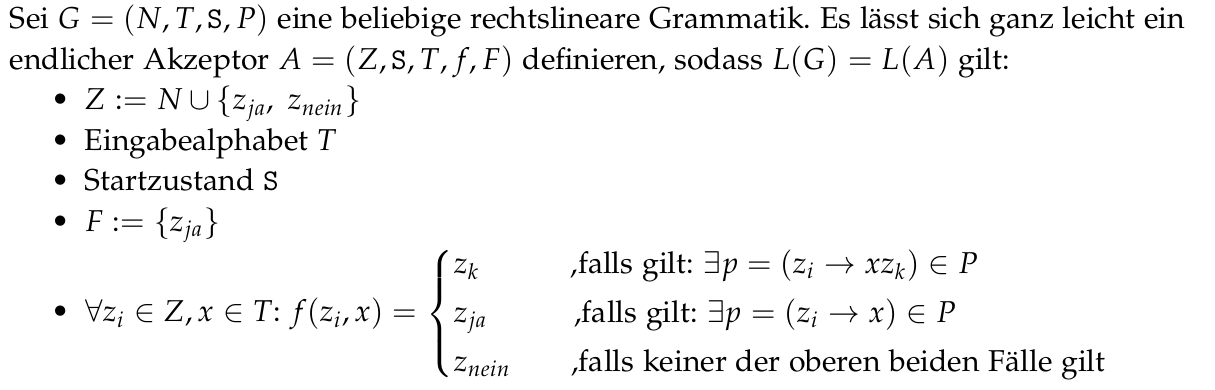
\includegraphics[width=\textwidth,height=\textheight,keepaspectratio]{UB10_2.png}
	\begin{itemize}[<+->]
		\item[b)] Wie kann die oben vorgestellte Konstruktion erweitert werden, sodass Produktionen, bei denen mehrere Terminalsymbole erzeugt werden, in A ebenfalls korrekt abgebildet werden? Beschreiben Sie die Ergänzung formal korrekt und zeichnen Sie als Beispiel das Resultat (ausschließlich) für die Produktion $(S \to \word{abab}A)$. Gehen Sie dabei von $T = \{a,b,c\}$ aus.
	\end{itemize}
\end{frame}


\framePrevEpisode

\begin{frame}{Algorithmen}
	\begin{block}{Definition}
		Ein Algorithmus ist...
		\begin{itemize}
			\item Eine endliche Beschreibung
			\item aus elementaren Anweisungen, 
			\item die deterministisch ($=$ ohne Zufall!) ausgeführt werden.\\
				{\small (Manchmal auch gemischt mit (Pseudo-)Zufallselementen)}
			\item Eine endliche Eingabe gibt endliche Ausgabe...
			\item in endlich vielen Schritten.
			\item Das funktioniert für beliebig große Eingaben und
			\item ist nachvollziehbar bzw. verständlich.
		\end{itemize}
	\end{block}
	\pause
	Woher wissen wir, ob ein Algorithmus korrekt ist? \pause \impl Hoare-Kalkül
\end{frame}

%\begin{frame}[t]{Wahr oder Falsch?}
%	\FalseQuestionE{Das (komplizierte) Master-Theorem kann man immer anwenden.}{ Nur bei rekursiven Algorithmen, bei denen das Problem in gleich große Teilprobleme aufgeteilt wird.}
%	\FalseQuestionE{Jeder Moore-Automat kann in einen Mealy-Automaten umgewandelt werden, der für jedes Wort die gleiche Ausgabe produziert.}{ Für das leere Wort kann ein Mealy-Automat niemals eine Ausgabe produzieren.}
%	\TrueQuestionE{Endliche Akzeptoren sind Moore-Automaten mit dem Ausgabealphabet $\{\word 0,\word 1\}$.}{}
%	\FalseQuestionE{Mit endlichen Automaten kann jede beliebige Sprache erkannt \\ werden.}{Tatsächlich ist die Menge der akzeptierbaren Sprachen sogar sehr eingeschränkt.}	
%\end{frame}

\renewcommand{\assert}[1]{\hoareassert{#1}}
\renewcommand{\kw}[1]{\textbf{#1}}

\section{Algorithmen: Hoare-Kalkül}

\subsection{Algorithmen}
\mycomment{%in last tut
	\begin{frame}{Algorithmen}
		\begin{block}{Definition}
			Ein Algorithmus ist...
			\begin{itemize}[<+->]
				\item Eine endliche Beschreibung
				\item aus elementaren Anweisungen, 
				\item die deterministisch ($=$ ohne Zufall!) ausgeführt werden.\\
					{\small (Manchmal auch gemischt mit (Pseudo-)Zufallselementen)}
				\item Eine endliche Eingabe gibt endliche Ausgabe...
				\item in endlich vielen Schritten.
				\item Das funktioniert für beliebig große Eingaben und
				\item ist nachvollziehbar bzw. verständlich.
			\end{itemize}
		\end{block}
		\pause[8]
		Woher wissen wir, ob ein Algorithmus korrekt ist?
	\end{frame}

	\begin{frame}{Korrektheit}
		Einige Algorithmen haben besonders hohe Anforderungen an ihre Korrektheit:
		Banking-Server, Airbag-Steuerprogramm, Herzschrittmacher, ...
		\bigskip

		
		Korrektheit garantieren?\pause
		\begin{itemize}
			\item Testen? \pause Was, wenn wir einen Sonderfall vergessen? \pause
			\item Alle Eingaben testen? \pause Oft nicht möglich. \pause
			\item Formal beweisen: \textbf{Hoare-Kalkül} \pause
		\end{itemize}
		
		\begin{block}{In der Praxis}
			Theoretisch müsste die komplette Werkzeugkette bewiesen werden:
			Programm, Compiler, Prozessor...\\
			Oft wird bei Compilern nur “Proven in use” benutzt: Compiler, bei
			denen seit Jahren keine Fehler gefunden wurden.
		\end{block}
		
	\end{frame}
}
\subsection{Hoare-Kalkül}
\begin{frame}{Der Hoare-Kalkül}
	\begin{block}{Definition}
		Ein \emph{Hoare-Tripel} ist ein Tripel $\set{P}\ S \ \set{Q}$ mit einem Programmstück $S$ und prädikatenlogischen \emph{Zusicherungen} $P,Q$.
	\end{block}
	\pause
	$P = $ Vorbedingung vor der Ausführung \\
	$Q = $ Nachbedingung nach der Ausführung\\
	$S = $ Programmstück
	
	\pause
	\bigskip
	Dabei: Wir betrachten nur \enquote{relevante} Interpretationen:
	\begin{itemize}[<+->]
		\item Fester Grundbereich (explizit angegeben oder implizit ableitbar)
		\item Funktionen und Relationen \enquote{wie üblich} interpretiert.
		\item Konstanten beliebig, als \enquote{Eingabe} des Programms.\\
		Muss also für alle Möglichkeiten (also Eingaben) gelten.
	\end{itemize}
\end{frame}

%TODO
\begin{frame}{Der Hoare-Kalkül}
	\begin{block}{Definition}
		Ein Hoare-Tripel $\htr{P}{S}{Q}$ ist \textbf{gültig}, wenn für jede relevante Interpretation $I$ und jede Variablenbelegung $\beta$ gilt:\\
		Wenn vor der Ausführung $\val_{D,I,\beta}(P)=\W$ ist und die Ausführung von $S$ für $I$ und $\beta$ mit der neuen Variablenbelegung $\beta'$ endet, dann gilt anschließend auch $\val_{D,I,\beta'}(Q)=\W$. \\
		\medskip
		Auf Deutsch: \\
		$\htr{P}{S}{Q}$ ist \textbf{gültig} \Gdw Wenn anfangs $P$ gilt, wir $S$ ausführen und dann zum Schluss $Q$ gilt.
	\end{block}
\end{frame}

\begin{frame}{Hoare-Tripel}
	\begin{Beispiel}
		\begin{columns}[T] 
			\begin{column}[T]{.4\textwidth} 
				$\assert{x = 5}$ \\
				$x \gets x + 1$ \\
				$\assert{x = 6}$ \\
				ist gültig.  \\
				
				\bigskip
				$\assert{x = 5}$ \\
				$x \gets x + 1$ \\
				$\assert{x = 42}$ \\
				ist nicht gültig.
			\end{column}
			\begin{column}[T]{.4\textwidth} 
				\pause
				$\assert{z = 5}$ \\
				$x \gets x + 1$ \\
				$\assert{z = 5}$ \\
				ist gültig.  \\
				
				
				\bigskip
				$\assert{x = x}$ \\
				$\kw{while } 1 = 1 \kw{ do } x \gets x + 1 \kw{ od}$ \\
				$\assert{\W = \F}$ \\
				ist gültig (Q wird nie erreicht).
			\end{column}
		\end{columns}
	\end{Beispiel}
	\medskip
	\pause
	\begin{block}{Hoare-Kalkül}
		Der \emph{Hoare-Kalkül} definiert Regeln, wie gültige \emph{Hoare-Tripel} schrittweise aus Axiomen abgeleitet werden können.
	\end{block}
\end{frame}


\begin{frame}{HT-A}
	\begin{block} {Axiom HT-A \quad „Assignment“}
		$$ \{\sigma_{\{\text{x/E}\}} (Q)\} \quad x \leftarrow E \quad \{Q\} $$
	\end{block}
	\pause
	Nach einer Zuweisung gilt jede Aussage für die Variable, welche vorher für die rechte Seite der Zuweisung galt.
	\begin{itemize}
		\item $\sigma_{\{\text{x/E}\}} (Q) $ ist die Aussage, die dadurch entsteht, dass man in Q jedes freie Vorkommen von x durch E ersetzt.
		\item \textbf{Achtung}: $\sigma_{\{\text{x/E}\}}$ muss kollisionfrei sein!
	\end{itemize}
	
	\begin{Beispiel}
		$\{ x + 1 = 43\} \ y \gets x + 1\ \{y = 43 \}$ ist gültig. \pause (Bzw. umgeformt \\
		$\{ x = 42 \} \ y \gets x + 1\ \{y = 43 \}$).
	\end{Beispiel}
	
\end{frame}

\begin{frame}{HT-E}
	\begin{block}{Regel HT-E}
		Wenn $\{P\}\ S\ \{Q\}$ gültig ist, dann auch $\{P'\}\ S\ \{Q'\}$ mit $P' \impl P$ und $Q \impl  Q'$.
	\end{block}
	\pause
	Heißt: Vorbedingungen können stärker, Nachbedingungen können schwächer werden.

	\begin{Beispiel}
		Aus $\{ x = 41\} \ x \gets x + 1\ \{x = 42 \}$ können wir \\
		$\{ x + y = 42 \land y = 1 \} \ x \gets x + 1\ \{x \in \R \}$ ableiten.
	\end{Beispiel}
\end{frame}

\begin{frame}{HT-S}
	\begin{block}{Regel HT-S \quad „Sequence“}
		Wenn $\{P\}\ S_1\ \{Q\}$ und $\{Q\}\ S_2\ \{R\}$ gültig sind, dann auch $\{P\}\ S_1;  S_2\ \{R\}$. 
	\end{block}
	\pause
	\impl Hoare-Tripel können transitiv zusammengefasst werden.
\end{frame}

\begin{frame}
	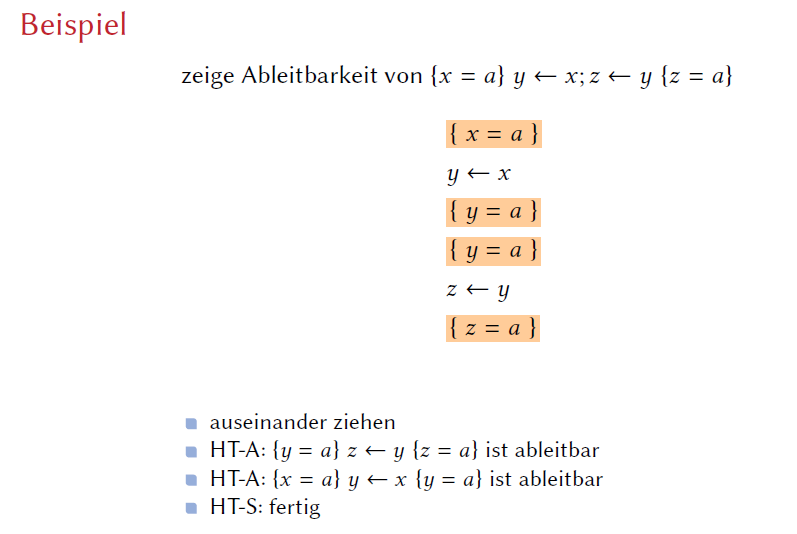
\includegraphics[scale=0.5]{hoare/bsp1}
\end{frame}

\begin{frame}{HT-I}
	\begin{minipage}{0.4\linewidth}
		\begin{align*}
			&\assert{ P } \\
			& \textbf{if } B \textbf{ then} \\
			&\hspace{2em} \assert{ P \wedge B } \\
			&\hspace{2em} S_1 \\
			&\hspace{2em} \assert{ Q }\\
			&\textbf{else} \\
			&\hspace{2em} \assert{ P \wedge \neg B } \\
			&\hspace{2em} S_2 \\
			&\hspace{2em} \assert{ Q }  \\
			&\textbf{fi}\\
			&\assert{Q }
		\end{align*}
	\end{minipage}
	\begin{minipage}{0.55\linewidth}
		\begin{block}{Regel HT-I \quad „If“}
			$\textbf{if } B\text{ } \textbf{ then } S_1 \textbf{ else } S_2 \textbf{ fi}$
			\smallskip
			\begin{itemize}
				\item Wenn $\{ P \wedge B \}\ S_1\ \{ Q \}$ gültig 
				\item und $\{ P \wedge \neg B \}\ S_2\ \{ Q \}$ gültig
				\item dann auch \\ $\{ P \} \textbf{ if } B \textbf{ then } S_1 \textbf{ else } S_2 \textbf{ fi } \{ Q \} $ gültig
			\end{itemize}
		\end{block}
%		\emph{HT4 : } $\textbf{if } B\text{ } \textbf{then } S_1 \textbf{ else } S_2 \textbf{ fi}$
%		\begin{itemize}
%			\item Wenn $\{ P \wedge B \} S_1 \{ Q \}$ gültig 
%			\item Wenn $\{ P \wedge \neg B \} S_2 \{ Q \}$ gültig
%			\item dann auch $\{ P \} \textbf{ if } B \textbf{ then } S_1 \textbf{ else } S_2 \textbf{ fi} \{ Q \} $ gültig
%		\end{itemize}
	\end{minipage}
\end{frame}

\begin{frame}{Beispiel: Berechnung von $\vert x \vert$}
	
	
	\begin{minipage}{0.4\linewidth}
		Erinnerung:
		\vspace{-.6\baselineskip}
		\begin{align*}
		&\assert{ P } \\
		& \textbf{if } B \textbf{ then} \\
		&\hspace{2em} \assert{ P \wedge B } \\
		&\hspace{2em} S_1 \\
		&\hspace{2em} \assert{ Q }\\
		&\textbf{else} \\
		&\hspace{2em} \assert{ P \wedge \neg B } \\
		&\hspace{2em} S_2 \\
		&\hspace{2em} \assert{ Q }  \\
		&\textbf{fi}\\
		&\assert{Q }
		\end{align*}
	\end{minipage}
	\begin{minipage}{0.4\linewidth}
		\begin{align*}
		&\assert{ x \in\R} \\
		&\textbf{if } x < 0 \textbf{ then } \\
		&\hspace{2em} \assert{ \visible<6->{ x\in\R\wedge x < 0 } } \\
		&\hspace{2em} \assert{ \visible<5->{ {-x} = \vert x \vert } } \\
		&\hspace{2em}  z \gets -x   \\
		&\hspace{2em} \assert{ \visible<2->{ z = \vert x \vert } } \\
		&\textbf{else} \\
		&\hspace{2em} \assert{ \visible<4->{ x\in\R\wedge x\geq 0 } } \\
		&\hspace{2em} \assert{ \visible<3->{ x = \vert x \vert } } \\
		&\hspace{2em} z \gets x \\
		&\hspace{2em} \assert{ \visible<2->{ z = \vert x \vert } } \\
		&\textbf{fi} \\
		&\assert{ z = \vert x \vert } 
		\end{align*}
	\end{minipage}
\end{frame}

\begin{frame}{Aufgabe}
	\vspace{-10mm}
	\begin{align*}
	&\assert{x=a \land y=b}  \\
	&\kw{if } x>y \kw{ then } \\
	&\hspace{2em} \assert{ \dots\ } \\
	&\hspace{2em}  z \gets y  \\
	&\hspace{2em} \assert{ \dots\ } \\
	&\kw{else } \\
	&\hspace{2em} \assert{ \dots\ } \\
	&\hspace{2em}  z \gets x  \\
	&\hspace{2em} \assert{ \dots\ } \\
	&\kw{fi } \\
	&\assert{z=\min(a,b)}
	\end{align*}
\end{frame}

\begin{frame}{Lösung}	
	\vspace{-2.5\baselineskip}
	\begin{alignat*}{2}
	&\assert{x=a \land y=b}  \\
	&\kw{if } x>y \kw{ then } \\
	&\hspace{2em} \assert{x=a \land y=b \land x>y} \\
	&\hspace{2em} \assert{y=\min(a,b)} \\
	&\hspace{2em}  z \gets y  \\
	&\hspace{2em} \assert{z=\min(a,b)} \\
	&\kw{else } \\
	&\hspace{2em} \assert{x=a \land y=b \land  \lnot (x>y)} \\
	&\hspace{2em} \assert{x=\min(a,b)} \\
	&\hspace{2em}  z \gets x  \\
	&\hspace{2em} \assert{z=\min(a,b)} \\
	&\kw{fi } \\
	&\assert{z=\min(a,b)}
	\end{alignat*}
\end{frame}


\mycomment{
%TODO: Lösung!!!
\begin{frame}{Jetzt seid ihr dran}
	\begin{align*}
	& z \gets x + y \\
	& z \gets z / 2 \\
	&\textbf{if } x \mod 2 = 0 \textbf{ then } \\
	&\hspace{2em} y \gets x + x \\
	&\hspace{2em} y \gets y / 4 \\
	&\textbf{else} \\
	&\hspace{2em} y \gets x - 1 \\
	&\hspace{2em} y \gets y / 2 \\
	&\textbf{fi} \\
	& z \gets z \· y \\
	&\assert{ z = div_2(a) \· (a+b)/2 } % WTF is div_2 ? => (2 `div`) ? a, b vs. x, y?
	\end{align*}
\end{frame}	
}


%\begin{frame}
%	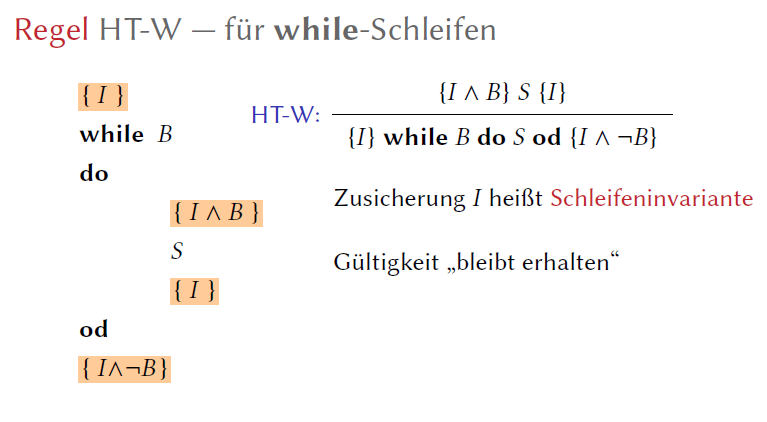
\includegraphics[scale=0.5]{hoare/htw}
%\end{frame}

\subsection{HT-W, Schleifeninvarianten}
\begin{frame}{HT-W}
	\begin{columns}[T] 
		\begin{column}[T]{.4\textwidth} 
			\vspace{-2\baselineskip}
			\begin{align*}
			&\assert{I} \q3uad \text{„Schleifeninvariante“} \\
			&\kw{while } B \kw{ do } \\
			&\qquad \assert{I \land B} \\
			&\qquad S \\
			&\qquad \assert{I} \\
			&\kw{od} \\
			&\assert{I \land \lnot B}
			\end{align*}
			\vspace{-1\baselineskip}
		\end{column}
		\begin{column}[T]{.4\textwidth} 
			\begin{block}{Regel HT-W \quad „While“}
				Wenn \htr{$I \land B$}{$S$}{$I$} gültig ist, dann ist auch die ganze \kw{while}-Schleife (s. links) gültig
			\end{block}
		\end{column}
	\end{columns}
	
	\pause
	\begin{block}{Schleifeninvarianten}
		\begin{itemize}
			\item sind Aussagen, die zu Beginn und Ende jedes Schleifendurchganges gültig sind
			\item helfen, die Korrektheit eines Programmes zu beweisen
			\item muss man ebenfalls beweisen 
			\item garantieren nicht die Korrektheit des Programms:\pause \\
			Terminierung der Schleife muss zusätzlich gezeigt werden! (nicht in GBI)
		\end{itemize}
	\end{block}
\end{frame}
	
\begin{frame}{Beispiel Schleifeninvarianten}
	\begin{columns}
	\begin{column}[T]{0.49\linewidth}
	\begin{align*}
		&\assert{x=a \land y=b}  \\
		&\assert{ \dots\ } \\
		&\kw{while } y\not=0 \kw{ do } \\
		&\qquad\assert{ \dots } \\
		&\qquad y \gets y-1 \\
		&\qquad\assert{ \dots } \\
		&\qquad x \gets x+1 \\
		&\qquad\assert{ \dots\ } \\
		&\kw{od } \\
		&\assert{ \dots\ } \\ \pause
		&\assert{x=a+b} \\
	\end{align*}
	\end{column} 
	
	\begin{column}[T]{0.5\linewidth}
		\visible<2->{
			\bigskip
			\begin{block}{Wertetabelle für $a=3$ und $b=4$}
				\centering
				\medskip
				\begin{tabular}{c|cc}	 
					Durchlauf $i$ & $x$ & $y$ \\ 
					\hline 
					0 & 3 & 4 \\
					1 & 4 & 3 \\
					2 & 5 & 2 \\
					3 & 6 & 1 \\
					4 & 7 & 0 \\
				\end{tabular}
			\end{block}
			\pause
			Schleifeninvariante: $$ x + y = a + b $$ 
		}
	\end{column}
	\end{columns}
\end{frame}

\begin{frame}{Beispiel Schleifeninvarianten – Lösung}
	\begin{minipage}{.4\linewidth}
		Erinnerung HT-W:
		\vspace{-.4\baselineskip}
		\begin{align*}
		&\assert{I}  \\
		&\kw{while } B \kw{ do } \\
		&\qquad \assert{I \land B} \\
		&\qquad S \\
		&\qquad \assert{I} \\
		&\kw{od} \\
		&\assert{I \land \lnot B}
		\end{align*}
	\end{minipage}
	\begin{minipage}{.4\linewidth}
		\begin{align*}
		&\assert{x=a \land y=b }  \\
		&\assert{ x+y=a+b }  \\
		&\kw{while } y\not=0 \kw{ do } \\
		&\qquad\assert{x+y=a+b \land y\not=0 }  \\
		&\qquad\assert{x+1+y-1=a+b } \\
		&\qquad y \gets y-1 \\
		&\qquad\assert{x+1+y = a+b} \\
		&\qquad x \gets x+1 \\
		&\qquad\assert{ x+y = a+b} \\
		&\kw{od } \\
		&\assert{ x+y = a+b \land y=0 } \\
		&\assert{x=a+b} \\
		\end{align*}
	\end{minipage}
	
\end{frame}

\begin{frame}{Exkurs: Schl.-Inv. mit Vollst. Induktion}
	Wir zeigen mit vollständiger Induktion die Gültigkeit der Schleifeninvariante. Dabei sei $i$ die Anzahl der bisher durchgelaufenen Schleifendurchläufe.\\
	
	\emph{Behauptung}: $$ \forall\ i \in \{0,...,b\} : x_i + y_i = a+b $$ \pause
	\begin{block}{Induktionsanfang}
		Für $i=0$ gilt $ x_0+y_0 = a+b $ nach Vorbedingung.
	\end{block} \pause 
	\begin{block}{Induktionsvorrausetzung}
		Für ein beliebig aber festes $i\in \{0,...,b\}$ gelte die Behauptung.
	\end{block}
\end{frame}

\begin{frame}{Exkurs: Schl.-Inv. mit Vollst. Induktion}
	\vspace{-2\baselineskip}
	\begin{align*}
	&\assert{x=a \land y=b}  \\
	&\assert{ x+y=a+b }\\
	&\kw{while } y\not=0 \kw{ do } \\
	&\qquad y \gets y-1 \\
	&\qquad x \gets x+1 \\
	&\kw{od } \\
	&\assert{x=a+b} \\
	\end{align*}
	\vspace{-2\baselineskip}
	\begin{block}{Induktionsschluss}
		Zu zeigen: $ x_{i+1} + y_{i+1} = a+b $ \pause
	%\vspace{-1.3\baselineskip}
		\begin{align*}
		x_{i+1}+y_{i+1} &= x_i +1 + y_i -1 \\
		&= x_i + y_i \\
		&\overset{IV}{=} a+b.
		\end{align*}
	\end{block}
\end{frame}

\begin{frame} {Weitere Beispiele}
	Weitere Beispiele findet ihr hier: Übung 8, WS 15/16
\end{frame}

\section{Quantitative Aspekte}

% TODO: Mehr und bessere Beispiele, generelle Überarbeitung (VL-Folien)

\subsection{Motivation}
\begin{frame}{Laufzeiten}
	Wir interessieren uns für Laufzeiten von Algorithmen.
	\pause
	\begin{itemize}
		\item Aber wie sollen wir die messen?
		\item Problem: Rechenzeit auf einem Supercomputing-Cluster nicht mit Rechenzeit auf einem IoT-Chip in der Waschmaschine vergleichbar
		\implitem Zählen der \enquote{ausgeführten Operationen} in Abhängigkeit von der Problemgröße $n$
		\item Noch ein Problem: Genaue Anzahlen sind seeehr schwierig zu bestimmen...
		\item[] ... und in vielen Fällen auch irrelevant
		\implitem konstante Faktoren ignorieren!
	\end{itemize}
\end{frame}

%% -----------------------------------------------------------------------------

\subsection{Definitionen}
\begin{frame}{Asymptotisches Wachstum}
	\begin{Definition}
		Zwei Funktionen $f,g: \N_0 \to \R_0^+$ wachsen asymptotisch gleich schnell, wenn es zwei Konstanten $c, c' \in \R^+$ gibt, so dass gilt $$\exists n_0 \in \N_0: \ \forall n \geq n_0: \ c \* f(n) \leq g(n) \leq c' \* f(n) $$
		Man schreibt dafür 
		\begin{align*}
			f &\asymp g \\
			\textbf{oder} \quad f(n) &\asymp g(n) 
			% Hashtag: „n^2“ ist ein Term und keine Funktion etc... Man müsse doch [n \mapsto n^2] schreiben... VL erlaubt ersteres aber auch.
		\end{align*}
	\end{Definition} \pause
	Diese Relation ist eine Äquivalenzrelation!
\end{frame}

\begin{frame}{Landau-Notation I}
	\begin{Definition}
		$\Theta(f)$ ist die Menge aller Funktionen $g$, die asymptotisch genauso schnell wachsen wie $f$, also $$\Theta(f) := \{ g \mid f \asymp g \}$$
	\end{Definition}
	
	\medskip
	\only<1|handout:1>{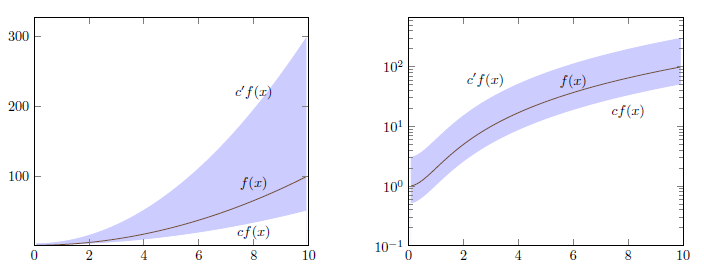
\includegraphics[scale=0.6]{laufzeit/theta1}}
	\only<2|handout:2>{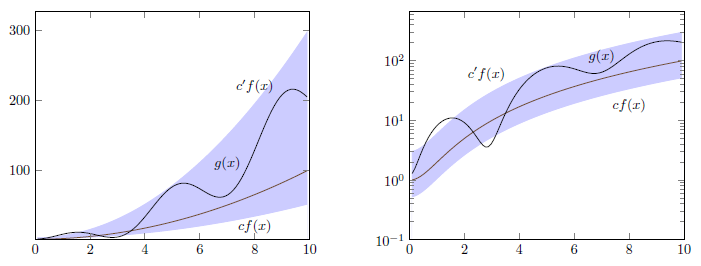
\includegraphics[scale=0.6]{laufzeit/theta2}}
\end{frame}

\begin{frame}{Beispiel 1}
	Seien \quad $f(n) := 2 \cdot n^2 + n, \qquad g(n) := n^2.$ \\
	\textbf{Behauptung:} \quad $ f \in \Th{g} $. \\ 
	\medskip \pause
	\textbf{Beweis:} \quad Wir suchen $n_0, c, c'$ mit $\forall n \geq n_0: \ c \* g(n) \leq f(n) \leq c' \* g(n) $.
	\smallskip \pause
	
	Sei $n \geq 1$, so gilt: \pause 
	\begin{align*}
	f(n) &= 2 \cdot n^2 + n \leq 2 \cdot n^2 + n^2 = 3 \cdot n^2 = 3 \cdot g(n)\quad \text{ und} \\ 
	\visible<5->{f(n) &= 2 \cdot n^2 + n \geq 2 \cdot n^2 = 2 \cdot g(n).}
	\end{align*}
	\pause % I hate you, LaTeX. -.-
	Mit $c := 2$, \, $c' := 3$,\, $n_0 := 1$ ist die Bedingung erfüllt. \qed \pause
	
	\begin{block}{Quiz}
		\TrueQuestion{$n^{100} + 10^9 n^{99} \in \Th{n^{100}}$}
		\FalseQuestion{$2^n \in \Th{n^2}$}
	\end{block}
\end{frame}

\begin{frame}{Beispiel 2}
	\textbf{Behauptung:} \quad $  \sin(n) + 2 \elem \Th{1} $ \\ \medskip \pause
	\textbf{Beweis:} \quad Wähle $c := 1, \, c' := 3, \, n_0 := 0$.  \quad Dann gilt $\forall n \geq n_0$: \\
	\begin{align*}
	c \* 1 = 1 &\leq \sin(n) + 2 \leq 3 = c' \* 1 \\
	\text{\Gdw} \qquad  -1 &\leq \sin(n) \leq 1. \qed
	\end{align*}
	\pause
	\Impl Der Sinus ist also „ungefähr“ konstant\only<handout>{ (wenn man seine Brille absetzt \smiley)}.
\end{frame}

\begin{frame}{Asymptotisches Wachstum}
	\begin{Definition}
		Für zwei Funktionen $f,g: \N_0 \to \R_0^+$ definiert man:
		$$g \preceq f \Gdw \exists c \in \R^+ \ \exists n_0 \in \N_0 \ \forall n \geq n_0: \ g(n) \leq c \* f(n)$$
		$$g \succeq f \Gdw \exists c \in \R^+ \ \exists n_0 \in \N_0 \ \forall n \geq n_0: \ g(n) \geq c \* f(n)$$
		(Schreibe analog auch $g(n) \preceq f(n)$ etc.)
	\end{Definition} \pause
	Diese Relationen sind \textbf{keine} Äquivalenzrelationen!
\end{frame}

\begin{frame}[t]{} % erased title due to \includepdf madness... I guess it's not that important anyway. Tags: fake title faketitle include pdf frametitle
	\fakeframetitle{Landau-Notation II}
	\begin{Definition}
		$\Oh{f}$ ist die Menge aller Funktionen $g$, die asymptotisch höchstens so schnell wachsen wie $f$, also $$\Oh{f} := \{ g \mid g \preceq f \}$$
		$\Om{f}$ ist die Menge aller Funktionen $g$, die asymptotisch mindestens so schnell wachsen wie $f$, also $$\Om{f} := \{ g \mid g \succeq f \}$$
	\end{Definition} \pause
	\impl $O$ ist eine Abschätzung nach oben. $\Omega$ ist eine Abschätzung nach unten.
\end{frame}


%\setbeamercolor{background canvas}{bg=}
%
\includepdf[pages=15]{U11.pdf}

\mycomment{ % let's not even teach them that this exists. Mentioning it in the lecture is enough
\begin{frame}{Eine katastrophale Schreibweise}
	Manchmal (häufig) sieht man auch das, \textbf{NICHT VERWENDEN}:
	$$f = \Theta(g) \qquad h = \Oh{n^3} \qquad k = \Omega(f + g)$$
	\pause
	Dabei das „$=$“ immer als „$\in$“ lesen!
\end{frame}
}

\begin{frame}[t]{} % fake title
	\fakeframetitle{Aufgabe: Inklusionen}
	Ordnet folgende Funktionen nach asymptotischem Wachstum an:
	\begin{itemize}
		\item Identität $f(x) = x$
		\item Konstante Funktion $f(x) = c$
		\item Wurzel
		\item Exponentialfunktion
		\item Logarithmus
	\end{itemize}
\end{frame}

%% Übung: Asymptotische Visualisierungen verschiedener Funktionen
\setbeamercolor{background canvas}{bg=}

\includepdf[pages={5-10}]{U11.pdf}

%\begin{frame}
%	\frametitle{Grenzwertabschätzung}
%	Wir können das auch anders schreiben:
%	\begin{align*}
%	f \in O(g) \qquad &\iff & \qquad 0 \leq  \limsup \limits_{n \to \infty} \frac{f(n)}{g(n)} < \infty \\
%	f \in \Omega(g) \qquad &\iff & \qquad 0 < \liminf  \limits_{n \to \infty} \frac{f(n)}{g(n)} \leq \infty \\
%	f \in \Theta(g) \qquad & \iff & \qquad 0 <  \liminf  \limits_{n \to \infty} \frac{f(n)}{g(n)} \leq  \limsup \limits_{n \to \infty} \frac{f(n)}{g(n)} < \infty
%	\end{align*} \pause
%	Oftmals existiert sogar $\lim$ und wir können $\liminf$ und $\limsup$ vergessen!
%\end{frame}
%
%\begin{frame}{Satz von L'Hospital}
%	\begin{block}{Satz}
%		Gegeben sei $$ \limes{x\to x_0} \frac{f(x)}{g(x)} $$ mit $$ \limes{x\to x_0} f(x) = \limes{x\to x_0} g(x) = 0 \vee \limes{x\to x_0} f(x) = \limes{x\to x_0} g(x) = \infty $$ 
%		Dann gilt 
%		$$ \limes{x\to x_0} \frac{f(x)}{g(x)} = \limes{x\to x_0} \frac{f'(x)}{g'(x)}   $$ mit 
%		$$ f'(x_0) = \left. \frac{\partial f(x)}{\partial x} \right|_{x=x_0} $$ 
%	\end{block}
%\end{frame}
%
%\begin{frame}{Beispiele}
%	Gilt $$ \log n \in \O \left(\sqrt{n}\right) $$ \pause 
%	Betrachte
%	\begin{align*}
%		\limes{n\to\infty} \log n &= \infty \\
%		\limes{n\to\infty} \sqrt{n} &= \infty \\
%		\frac{\partial \log n}{\partial n} &= \frac{1}{n} \\
%		\frac{\partial \sqrt{n}}{\partial n} &= \frac{1}{2} \frac{1}{\sqrt{n}} \\
%		\limes{n\to\infty} \frac{\log n}{\sqrt{n}} &= \limes{n\to\infty} \frac{\frac{1}{n}}{\frac{1}{2} \frac{1}{\sqrt{n}}} \\
%		&= 2 \limes{n\to\infty} \frac{\sqrt{n}}{n}  = 2 \limes{n\to\infty} \frac{1}{\sqrt{n}} = 0 
%	\end{align*}
%\end{frame}

%\subsection{Beispiele}
%\begin{frame}{Polynome}
%	Betrachten wir zwei Polynome $f(n) = n^4 + n^3$ und $g(n) = n^2$: \\
%	Der Quotient $$\frac{f(n)}{g(n)} = \frac{n^4 + n^3}{n^2} = n^2 + n \to \infty$$ Also ist $\lim f/g > 0$ und damit $$g \in O(f) \qquad f \in \Omega(g)$$ aber $\lim f/g = \infty$ also $$f \not \in O(g) \qquad g \not \in \Omega(f)$$ und vor allem $$f \not \in \Theta(g)$$
%\end{frame}

\begin{frame}{Logarithmen}
	\only<handout:0>{Informatiker LIEBEN Logarithmen...\\}
	\begin{block}{Einige Rechenregeln}
		\begin{align*}
			a^{\log_a n} &= n\\
			\visible<2-|handout:1>{\log_b (n \cdot m) &= \log_b n + \log_b m\\ 
			\log_b n^a &= a \cdot \log_b n\\}
			\visible<3-|handout:1>{a^{\log_b n} &= n^{\log_b a}}
		\end{align*}
	\end{block}
\end{frame}

\begin{frame}{Logarithmen}
	\begin{block}{Lemma}
		$$a^{\log_b n} = n^{\log_b a}$$
	\end{block} \pause

	\begin{block}{Herleitung}
		\begin{align*}
			a^{\log_b n} &= \left( b ^{\log_b a} \right) ^{\log_b n}\\
						 &= b^{\log_b a \, \cdot \, \log_b n}\\
						 &= \left( b^{\log_b n} \right) ^{\log_b a}\\
						 &= n^{\log_b a}
		\end{align*}
	\end{block}
\end{frame}

\begin{frame}{Logarithmen: Die Basis ist egal}
	\begin{block}{Lemma}
		$$ \log_a n \in \Th{\log_b n} $$
	\end{block}
	
	\begin{block}{Herleitung}
		Es gilt $$n = a^{\log_a n}$$ \pause
		Daraus ergibt sich: $$ \log_b n = \log_b \left(a^{\log_a n}\right) = \log_a n \; \cdot \log_b a $$ \pause 
		Setze $c = c' = \log_b a$, dann ist $$c \* \log_a n \leq \log_b n \leq c' \* \log_a n.$$
	\end{block}
\end{frame}

\begin{frame}{Logarithmen: Übung}
	\begin{block}{Einige Rechenregeln}
		\begin{align*}
			a^{\log_a n} &= n\\
			\log_b (n \cdot m) &= \log_b n + \log_b m\\ 
			\log_b n^a &= a \cdot \log_b n\\
			a^{\log_b n} &= n^{\log_b a}
		\end{align*}
	\end{block}

	\begin{block}{Aufgabe}
		\begin{align*}
			\log_5(25 \cdot 125) &= \visible<2->{\log_5(25) + \log_5(125) = 2+3 = 5}\\
			16^{\log_4(5)} &= \visible<3->{5^{\log_4(16)} = 5^2 = 25}
		\end{align*}
	\end{block}
\end{frame}

\begin{frame}{Rechenregeln (I)}
	Einige Rechenregeln im $O$-Kalkül
	\begin{itemize}[<+->]
		\item Für $a > 0$ ist $a \cdot f \in \Th{f}$ 
		\item Für Konstanten $c, d \geq 0$ gilt: \\ 
			\quad $f(n) \in \Oh{g(n)} \Impl f(n) + c \in \Oh{g(n) + d}$ \\
			\quad $f(n) \in \Om{g(n)} \Impl f(n) + c \in \Om{g(n) + d}$ \\
		\item Für $0 < a < b$ ist $n^a \preceq n^b$
		\item Für $a,b > 1$ ist $n^a \preceq b^n$ \qquad {\small (Exponentialfktnen. wachsen stärker als Polynome)}
		\item Für Polynome $f,g$ gilt: \\
			\quad $\mathop{\text{grad}} f = \mathop{\text{grad}} g \iff f \asymp g $
		\item Für $a,b > 0$ gilt $\log_a(n) \in \Theta(\log_b n)$
		
	\end{itemize}
\end{frame}


\begin{frame}{Rechenregeln (II)}
	Weitere Rechenregeln im $O$-Kalkül:
	\begin{itemize}[<+->]
		\item $f \in O(g) \iff g \in \Omega(f)$
		\item $\Theta(f) = O(f) \cap \Omega(f)$ und $f \asymp g \iff f \preceq g \wedge f \succeq g$ 
		\item $O(f_1) + O(f_2) = O(f_1 + f_2)$
		\item Wenn $g \in O(f)$, dann ist auch $O(g) \subseteq O(f)$ und $O(f + g) = O(f)$
	\end{itemize}

	\begin{block}{Kurze Aufgabe}
		Zeigt mit den Rechenregeln: Wenn $g\preceq f$, $h \succeq f$ und $h\in\Oh{g}$, dann ist $f \asymp g \asymp h$.
	\end{block}
\end{frame}

% TODO Aufgaben !!!!

%\subsection{Laufzeiten Angeben}
%
%\begin{frame}[fragile]
%	\frametitle{Algorithmus}
%		\verb+int x = 1;+ \\
%		\verb/for (int i = 0; i < n; i++) {/ \\
%		\verb+	x = a * x;+ \\
%		\verb+}+ \\
%		\verb+return(x);+ \\[1em]
%		 \pause
%	Was tut der? \pause Welche Laufzeit hat er?
%\end{frame}
%
%\begin{frame}[fragile]
%	\frametitle{Laufzeiten}
%		\verb+int x = 1;+ \\ \pause $O(1)$ \\ \pause
%		\verb/for (int i = 0; i < n; i++) {/ \\  \pause $O(1), O(1)$ \\ \pause
%		\verb+	x = a * x;+ \\  \pause $O(1)$ \\ \pause
%		\verb+}+ \\  \pause $n$-mal \\ \pause
%		\verb+return(x);+ \\  \pause $O(1)$ \\ \pause
%		 \pause
%		$$O(1 + n + n + 1) = O(n)$$
%\end{frame}


\begin{frame}	
	\begin{block}{Was ihr nun wissen solltet}
		\begin{itemize}
			\item Korrektheit von Algorithmen zeigen
			\item Asymptotisches Wachstum
		\end{itemize}
	\end{block}

	
	\begin{block}{Was nächstes Mal kommt}
		\begin{itemize}
			\item O-Kalkül - Rechnen
			\item Endlich: Graphen
			\item verschiedene Darstellungsformen von Graphen
		\end{itemize}
	\end{block}
\end{frame}

% TODO ?
%input{../Bloecke/StrukturelleInduktion}

%TODO replacement?
{\xkcdframe{1724}{Danke für eure Aufmerksamkeit! \smiley}{2.5}}
%\thasse{\lastframe{0.5}{0}{xkcd/proofs_1724.png}{https://www.xkcd.com/1724/}}

\slideThanks

\end{document}